
\section*{Introduction}

In the present work, we attempt to replicate the results of Young et al. 2001 ``Reproductive pair correlations and the clustering of organisms'' \cite{young_reproductive_2001}, an analysis of the formation of aggregates in an homogeneous environment mimicking marine turbulence. Using an individual-based model of independent, random-walking particles (also called ``brownian bugs''), they show that simple ecological processes such as birth and death in a turbulent and viscous flow leads to the formation of elongated clusters and therefore departure from the usual, homogeneous solution of the advection-diffusion-reaction equation for a large population. This could explain the observed patchiness of communities such as the phytoplankton. \\

Our first interest in this paper was mostly driven by a major ecological question: the so-called paradox of the plankton \citep{hutchinson_paradox_1961}, i.e. the surprising diversity of phytoplankton species competing for the same resources in a seemingly homogeneous environment. Aggregation of phytoplanktonic organisms, observed at macro- to micro-scales \citep{lovejoy_universal_2001,pinel2007spatial}, could explain part of their coexistence, as spatial clustering can help reduce interspecific interactions \citep{font-munoz_advection_2017} and/or allow species to benefit from different organic substrates \citep{seymour_resource_2009}. Due to their size, microphytoplankton organisms experience a mostly viscous environment in a laminar shear fields, with random, but homogeneous changes in directions due to turbulence \citep{peters_effects_2000}. Ecological phenomena as simple as growth and death, which occur at the phytoplankton scale, interact with these hydrodynamics processes and can lead to aggregates. In this context, a better understanding of the interactions between demographic stochasticity and environmental fluctuations at small scales could provide further explanation for the distribution and coexistence of these organisms in turbulent environments. \\

In this replication, we aim not only to replicate the main results of the paper, but also to clarify and develop the mathematical background behind the model main equations, with key inputs from co-author (and first author of the original paper), William Young. %If we add Bill, then he's included within ``our''
 
\section*{Methods}

\subsection*{Brownian bug model}
The brownian bug model is a discrete-time, individual-based model, here presented in its 2D formulation. Each particle is characterized by the vector of its Cartesian coordinates $\boldsymbol{x}=\begin{pmatrix} 
      x_1\\ 
      x_2 
\end{pmatrix}$ and its original position on the y-axis at $t=0$ (a child particle inherits this attribute), this last attribute being used only for representation purposes. Space is a $L\times L$ square with periodic boundary conditions. Each timestep, of duration $\tau$, is divided into three substeps: (1) demographic processes, (2) diffusion, and (3) advection. \\

(1) Demographic processes take place during the first substep. The discrete-time Markov chain of the brownian bug model can be approximated as a continuous-time spatial birth-death process (described in the Supplementary Material), also referred to in Young et al. \cite{young_reproductive_2001} as a Galton-Watson process. Each organism has a fixed probability ($p$) of reproducing, dying ($q$), or remaining unchanged ($1-p-q$). When an individual reproduces, a new organism appears on top of the parent. In the following, $p=q=0.5$.

(2) Diffusion is modeled as a brownian motion, i.e. $\boldsymbol{x'}_k(t)=\boldsymbol{x}(t)+\delta\boldsymbol{x}(t)$ where each component of $\delta\boldsymbol{x}(t)$ follows a Gaussian distribution $\mathcal{N}(0,\Delta)$ where $D=\frac{\Delta^2}{2\tau}$ is the diffusivity. 

(3) The turbulent flow governing advective stirring follows the Pierrehumbert random map.

\begin{eqnarray}
 x_1(t+\tau)&=&x'_1(t)+(U\tau/2)\cos[kx'_2(t)+\phi(t)]\\
 x_2(t+\tau)&=&x'_2(t)+(U\tau/2)\cos[kx_1(t+\tau)+\theta(t)]
 \label{eq:pierrehumbert}
 \end{eqnarray}

 where $\phi(t)$ and $\theta(t)$ are random phases uniformly distributed between 0 and $2\pi$, $k=2\pi/L$ (in the rest of the paper, we use $k=2\pi$) and $U$ is the stretching parameter. \\
 
Unless otherwise specified, each simulation is initialized with $N_0=20,000$ particles uniformly distributed in a $1\times 1$ square and run for 1000 timesteps. 
 
% \subsection*{Relation with the advection-diffusion-reaction approximation} 
% In continuous time, the distribution of particles in conditions similar as those described in the brownian bug model can be approximated by the advection-diffusion-reaction (ADR) equation. 
% 
% \begin{equation}
% \frac{dC}{dt}=D\nabla^2 C+(\lambda-\mu)C
% \label{eq:ADR}
% \end{equation}
% 
% where $C$ is the concentration of particles, $\lambda$ is the growth rate ($\lambda=p/\tau$)  and $\mu$ is the death rate ($\mu=q/\tau$). When $\lambda=\mu$, the solution of eq. \ref{eq:ADR} is $C(\boldsymbol{x},t)=C_0$ where $C_0$ is the initial uniform concentration. To compare this theoretical distribution to the actual distribution, the brownian bug model is run without the advection component ($U=0$). While the brownian bug model is a discrete-time model, we consider $\tau \leftarrow 0.1$. \\
% 
% To assess the effect of the turbulent motion, the model is also run without its demographic component, but with advection and diffusion.
\subsection*{Pair correlation function G(r,t)}

The pair density function $G(\boldsymbol{x}_i,\boldsymbol{x}_j,t)$ is defined so that $G(\boldsymbol{x}_i,\boldsymbol{x}_j,t)dA_1dA_2$ is the probability of finding a pair of brownian bugs with one member in the area $dA_1$ around $\boldsymbol{x}_1$ and the other in the area $dA_2$ around $\boldsymbol{x}_2$. $G(\boldsymbol{r},t)$ is actually called the pair correlation function in \cite{young_reproductive_2001}. The radial density function $g(r,t)$ is defined as $G(\boldsymbol{x}_i,\boldsymbol{x}_j,t)=C^2g(r,t)$ with $r=|\boldsymbol{x}_i-\boldsymbol{x}_j|$. As the pair correlation disappear when $r\rightarrow\infty$, $g\rightarrow 1$. \\

\subsubsection*{Derivation of G(r,t)}

All details of the derivation of $G(r,t)$ are to be found in the Supplementary Material. We finally obtain:

\begin{equation}
\frac{\partial G}{\partial t}=2Dr^{1-d}\frac{\partial}{\partial r}\left(r^{d-1}\frac{\partial G}{\partial r}\right)+2(\lambda-\mu)G+\gamma r^{1-d}\frac{\partial}{\partial r}\left(r^{d+1}\frac{\partial G}{\partial r}\right)+2\lambda C\delta(\boldsymbol{x})\label{eq:eq_2_Young_total}
\end{equation}

where $\boldsymbol{x}$ is the position of the particle. \\

We focus on the case $d=2$ and $\lambda=\mu$, which means Eq.
(\ref{eq:eq_2_Young_total}) can be reduced to

\begin{equation}
\frac{\partial G}{\partial t}=\frac{2D}{r}\frac{\partial}{\partial r}\left(r\frac{\partial G}{\partial r}\right)+\frac{\gamma}{r}\frac{\partial}{\partial r}\left(r^{3}\frac{\partial G}{\partial r}\right)+2\lambda C\delta(\boldsymbol{x})\label{eq:eq_2_Young_reduced}
\end{equation}

The value of $\gamma$ is computed from simulations (see Supplementary Material).

\subsubsection*{Analytical solution with advection}

The analytical solutions of $G(r,t)$ with and without advection could only be found with the indications of WY. In the presence of advection ($\gamma\neq0$), a steady-state solution
can be found; without advection, there is no steady-state. 

\begin{align}
  &  \frac{2D}{r}\frac{\partial}{\partial r}\left(r\frac{\partial G}{\partial r}\right)+\frac{\gamma}{r}\frac{\partial}{\partial r}\left(r^{3}\frac{\partial G}{\partial r}\right)+2\lambda C\delta(\boldsymbol{x})\nonumber & = & & 0 \\
\Leftrightarrow & 2\pi r\left(\frac{2D}{r}\frac{\partial}{\partial r}\left(r\frac{\partial G}{\partial r}\right)+\frac{\gamma}{r}\frac{\partial}{\partial r}\left(r^{3}\frac{\partial G}{\partial r}\right)+2\lambda C\delta(\boldsymbol{x})\right)\nonumber & = & & 0 \\
 \Leftrightarrow  & 2\pi\left(2D\frac{\partial}{\partial r}\left(r\frac{\partial G}{\partial r}\right)+\gamma\frac{\partial}{\partial r}\left(r^{3}\frac{\partial G}{\partial r}\right)\right)+2\pi r2\lambda C\delta(\boldsymbol{x}) & = & & 0\label{eq:steady_state}
\end{align}

We can then integrate Eq. (\ref{eq:steady_state}) over a small
area centered on a particle, with radius $\rho$. Let us first note
that

\begin{align}
& \int_{\mathbb{R}^{2}}\delta(\boldsymbol{x})d^{2}\boldsymbol{x} & & = & & 1\nonumber \\
\Leftrightarrow & \int_{0}^{2\pi}\int_{0}^{\rho}\delta(r')\delta(\theta)r'dr'd\theta & & = & & 1\nonumber \\
\Leftrightarrow & 2\pi\int_{0}^{\rho}\delta(\boldsymbol{x'})r'dr' & & = & & 1\label{eq:delta_integration}
\end{align}

where $\boldsymbol{x'}$ is the equivalent of $\boldsymbol{x}$ in polar coordinates. 

Using Eq. (\ref{eq:steady_state}) and (\ref{eq:delta_integration}),
we can integrate between 0 and $\rho$, 

\begin{align}
 & & 0 & & = & & 2\pi\left(2D\rho\frac{\partial G}{\partial r}+\gamma\rho^{3}\frac{\partial G}{\partial r}\right)+2\lambda C\nonumber \\
\Leftrightarrow & & \frac{\partial G}{\partial r} & & = & & -\frac{1}{2\pi}\frac{2\lambda C}{2D\rho+\gamma\rho^{3}}\label{eq:deriv_G_r}
\end{align}

Eq. (\ref{eq:deriv_G_r}) can now be integrated between $\rho$ and $\infty$, knowing that $G(\infty)=C^{2}.$

\begin{equation}
 C^{2}-G(\rho) = -\frac{1}{2\pi}{\displaystyle \int_{\rho}^{\infty}}\frac{2\lambda C}{2Dr+\gamma r^{3}}dr\label{eq:deriv_G_r_int1}
\end{equation}

Using the variable change $u=2Dr+\gamma r^{3}$, the integral is equivalent
to $\int\frac{u'}{u}du$.

\begin{align}
 & C^{2}-G(\rho) & = & & -\frac{\lambda C}{2\pi}\frac{1}{4D}[\log(\gamma)-\log(\frac{2D}{r^{2}}+\gamma)]\label{eq:deriv_G_rint2}\\
\Leftrightarrow & G(\rho) & = & & \frac{\lambda C}{8\pi D}\log\left(\frac{2D+\gamma r^{2}}{\gamma r^{2}}\right)+C^{2}\label{eq:G_rho}
\end{align}

Finally, the pair correlation function $g=G/C^{2}$ is defined as

\begin{equation}
g=\frac{\lambda}{8\pi DC}\log\left(\frac{2D+\gamma r^{2}}{\gamma r^{2}}\right)+1
\end{equation}


\subsubsection*{Analytical solution without advection}

When $U=0$, $\gamma=0$ and there is no steady solution. We can get
back to Eq. (\ref{eq:eq_2_Young_reduced}). 

\begin{equation}
\frac{\partial G}{\partial t}=\frac{2D}{r}\frac{\partial}{\partial r}\left(r\frac{\partial G}{\partial r}\right)+2\lambda C\delta(\boldsymbol{x})\label{eq:g_without_advection}
\end{equation}

Assuming an isotropic environment (and switching to the polar coordinate system), this means

\begin{equation}
\frac{\partial G}{\partial t}-2D\Delta G=2\lambda C\delta(\boldsymbol{x})
\end{equation}

where $\Delta=\nabla^{2}$ is the Laplacian operator. \\

We therefore have 

\begin{equation}
\mathcal{L}G(\boldsymbol{x},t)=2\lambda C\delta(\boldsymbol{x})\label{eq:LG_lambda}
\end{equation}

where $\mathcal{L}$ is the linear differential operator $\partial_{t}-2D\Delta$. \\

We can use the Green's function H, defined with $\mathcal{L}H=\delta(\boldsymbol{x},t)=\delta(\boldsymbol{x})\delta(t)$. \\

By definition, we know that $G(y)=\int H(y,s)2\lambda C\delta(s)ds$
(where $y=(\boldsymbol{x},t)$) is a solution to Eq.(\ref{eq:LG_lambda}).

\begin{align}
 & G(\boldsymbol{x},t) & = & & 2\lambda C\int_{\mathbb{R}^{2}}\int_{0}^{t}H(\boldsymbol{x}-\boldsymbol{x}',t')\delta(\boldsymbol{x}')d^2\boldsymbol{x}'dt'\nonumber \\
\Leftrightarrow &  & = &  & 2\lambda C\int_{0}^{t}H(\boldsymbol{x},t')dt'\label{eq:g_int_H}
\end{align}

Eq.(\ref{eq:g_int_H}) can be used in Eq. (\ref{eq:g_without_advection}):

\begin{alignat}{3}
 & \frac{\partial}{\partial t}\left(2\lambda C\int_{0}^{t}H(\boldsymbol{x},t')dt'\right) & & = & & 2D2\lambda C\Delta\int_{0}^{t}H(\boldsymbol{x},t')dt'+2\lambda C\delta(\boldsymbol{x})\\
\Leftrightarrow & \int_{0}^{t}\left(\frac{\partial H(\boldsymbol{x},t')}{\partial t'}-2D\Delta H(\boldsymbol{x},t')\right)dt' & & = & & \delta(\boldsymbol{x})\\
\Leftrightarrow & \int_{0}^{t}\delta(\boldsymbol{x})\delta(t')dt' & & = & & \delta(\boldsymbol{x})
\end{alignat}

which is true. \\

A solution for the Green's function using $\mathcal{L}=\partial_{t}-2D\Delta$
in 2 dimensions is $$H(r,t)=\frac{1}{4\pi2Dt}\exp(\frac{-r^{2}}{4\times2Dt})$$. 

$G(r,t)$ can then be computed:

\begin{equation}
G(r,t)=2\lambda C\left[\frac{E_1 \left(\frac{r^{2}}{8Dt'}\right)}{8D\pi}\right]_{0}^{t}\label{eq:G_r_t}
\end{equation}

where $E_1$ is the exponential integral. Using $G(r,0)=C^{2}$ and
$\lim_{x\rightarrow+\infty}E_1=0$ in Eq. (\ref{eq:G_r_t}), 

\begin{equation}
G(r,t)=2\lambda C\frac{E_1\left(\frac{r^{2}}{8Dt}\right)}{8D\pi}+C^{2}
\end{equation}

\begin{equation}
\Leftrightarrow g(r,t)=\frac{2\lambda}{C}\frac{E_1\left(\frac{r^{2}}{8Dt}\right)}{8D\pi}+1
\end{equation}

\section*{Results}

We were able to reproduce the spatial distributions of brownian bugs in each case described in \cite{young_reproductive_2001}.\\

In Fig. \ref{fig:spatial_fig1}, the model has been run without the advection component and we can see the clumping of organisms due to demographic processes. In Fig. \ref{fig:spatial_fig2} a), the model has been run without its demographic component, but with advection and diffusion, confirming that hydrodynamics alone cannot ensure cluster formation, while in Fig.  \ref{fig:spatial_fig2} b), all processes are taken into account, in which case organisms form aggregates.

\begin{figure}[H]
\begin{center} 
 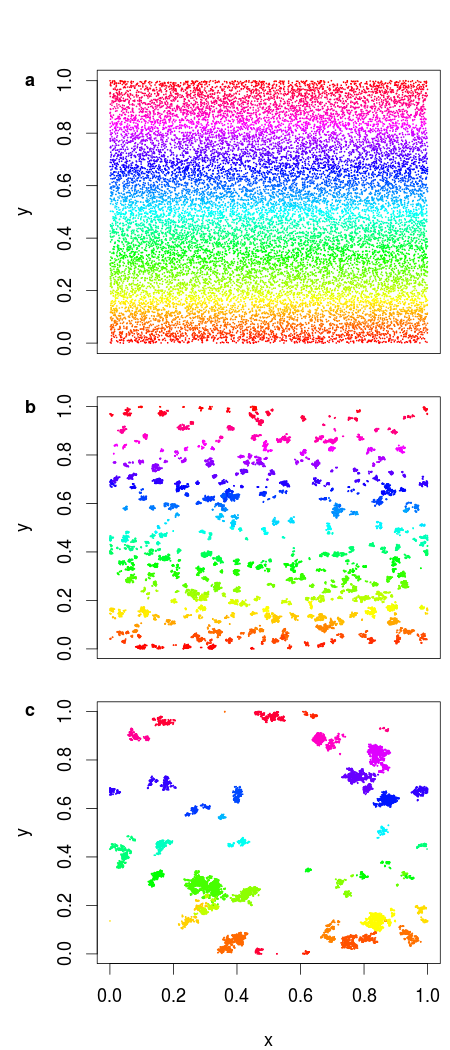
\includegraphics[width=0.49\textwidth]{../code/figure/spatial_distribution_Fig1.png}
  \caption{Distribution of brownian bugs at different times in a simulation with $\Delta=10^{-3}$ and $U=0$: initial conditions with a Poisson spatial distribution (a), $t=100\tau$ (b) and $t=1000\tau$ (c). Each particle is identified by a color which corresponds to the initial position on the y-axis of its ancestor at $t=0$.}
  \label{fig:spatial_fig1}
\end{center}
  \end{figure}

\begin{figure}[H]
\begin{center}
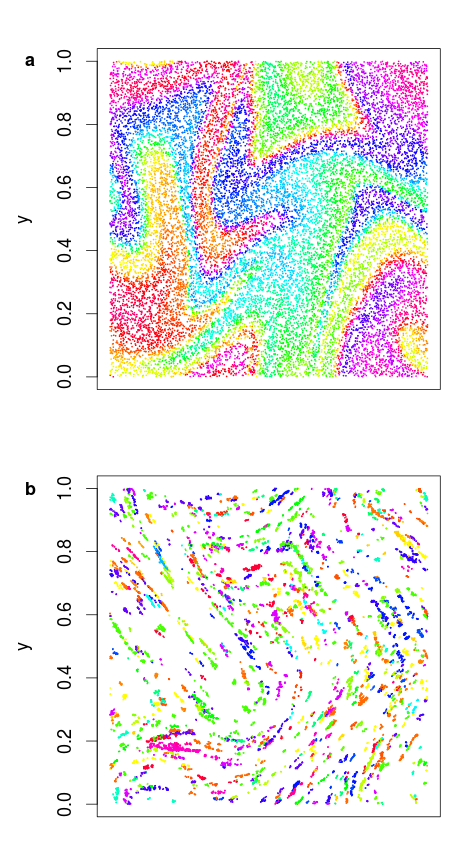
\includegraphics[width=0.49\textwidth]{../code/figure/spatial_distribution_Fig2.png}
  \caption{Distribution of brownian bugs with different processes in a simulation with $\Delta=10^{-3}$ and $U\tau/2=0.1$: without demographic processes at $t=30\tau$ (a), and with demographic processes at $t=1000\tau$ (b). Each particle is identified by a color which corresponds to the initial position on the y-axis of its ancestor at t=0.}
  \label{fig:spatial_fig2}
\end{center}
  \end{figure}
  
Fig. \ref{fig:pcf_Fig3} proved much more challenging. Retrieving the analytical solutions of eq. \ref{eq:eq_2_Young_reduced} could hardly be done without the inputs of WY. However, we also encountered issues when computing the pair correlation functions on simulations: for large values of $r/\Delta$, we observed zero values (absent pairs) of the pcf when $U=0$. Despite the missing values, we can confirm that simulated and analytical pcf match (Fig \ref{fig:pcf_Fig3}), with a slight underestimation by the simulations. The pcf also got closer to 1 than the predictions for larger values of $r$. %% F: predictions -> analytical predictions? 

\begin{figure}[H]
\begin{center}
 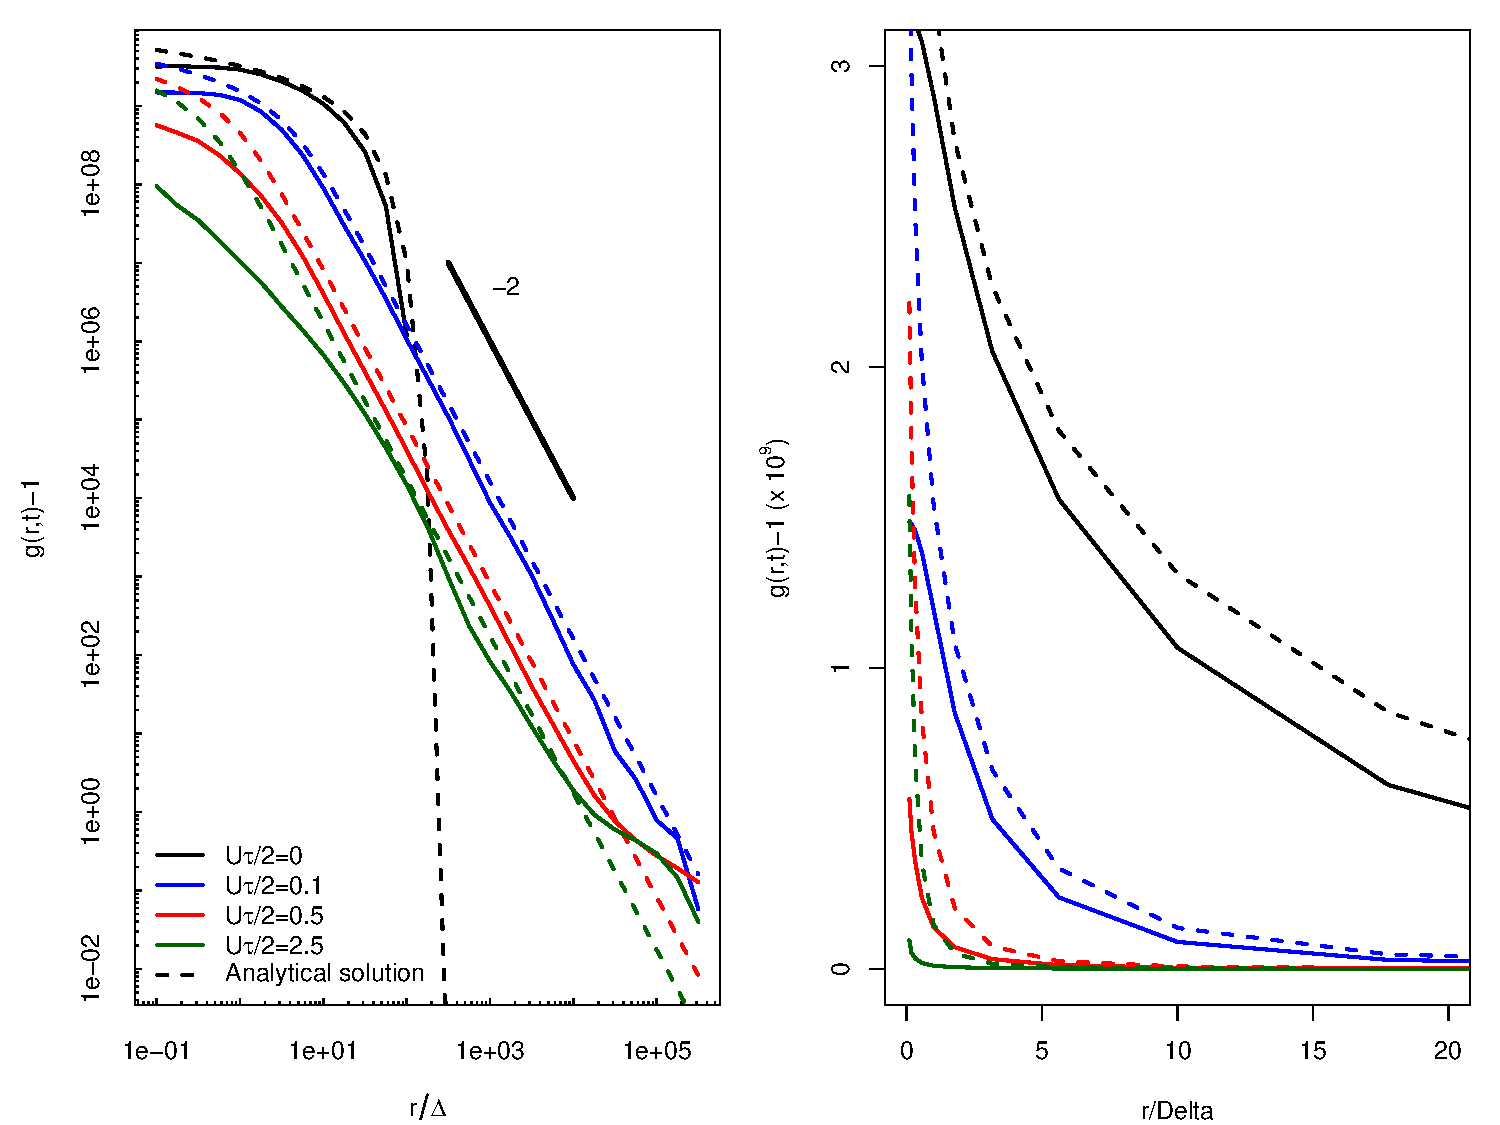
\includegraphics[width=0.99\textwidth]{../code/simulation/pcf_test_Utot_modif_dx_dp.pdf}
 \caption{Logarithmic (a) and linear (b) plots of $g(r,t)$ versus $r/\Delta$, with $\Delta=10^{-7}$ and $U\tau/2=0,0.1,0.5,2.5$ at $t=1000\tau$. Solid lines result from simulations, dotted lines correspond to analytical solutions and the solid grey line indicates the $r^{-2}$ scaling predicted by eq. \ref{eq:eq_2_Young_total}.}
  \label{fig:pcf_Fig3}
\end{center}
  \end{figure} 
 
\section*{Discussion}

We successfully replicated both the numerical results and analytical solutions of \citep{young_reproductive_2001}. Even though stochasticity prevents us from replicating exactly the same spatial point patterns as those seen in Fig. \ref{fig:spatial_fig1} and Fig. \ref{fig:spatial_fig2}, we considered the patterns to be close enough to validate the simulations. Fig. \ref{fig:pcf_Fig3} was also very close to the one shown in the original article, despite a slight underestimation.\\

The most challenging part of the replication was not actually to replicate the numerical results, but to find back the analytical expression of the pair density function $G(r,t)$ from first principle (this was briefly explained in words in the original article). WY provided the necessary mathematical steps to find the analytical solutions shown in Fig. \ref{fig:pcf_Fig3}. We hope that such additional mathematical derivations will help readers through both the original and replication articles. \\

The original article did not provide quantitative values exactly matching marine microbes ecology; we thus wondered about the time and spatial scales that could be used for a realistic phytoplankton model. The length of the square side, $L$, is defined as the Kolmogorov scale, that is the scale at which viscosity starts dominating turbulence. In the ocean, this value oscillates between 1 and 10 mm \citep{barton_impact_2014} (which corresponds to the value which was indicated by WY, i.e. 1 cm). %%[F: I am not sure I understand this, is it 1mm or 1cm? Do we say, ``corresponds roughly'' then?]
If we consider a phytoplankton doubling rate of 0.5-1 d$^{-1}$ \citep{bissinger_predicting_2008}, $p=0.5$ means that $\tau=0.25 - 0.5$ d. In this case, assuming we can write $U\tau/2=0.1L$ (the value used in Fig. \ref{fig:spatial_fig2}), $U\approx 5.5$ $10^{-5}$ cm.s$^{-1}$, which seems very low for the oceanic current (around 1-10 cm.s$^{-1}$ near the coast in \cite{font-munoz_advection_2017}, similar in the North Atlantic Ocean \citep{flatau_north_2003}). We should therefore have a lower reproduction probability $p$, if we wanted to keep the values of the other parameters. The diffusion coefficient can be hard to approximate. Brostr\"om \citep{brostrom_advection_2002} suggests a value of $10^{-8}$ m$^{2}$.s$^{-1}$, which would lead to $\Delta \approx 10^{-4}$. This is much higher from the value used in Fig. \ref{fig:pcf_Fig3} ($\Delta=10^{-7}$) but only one order of magnitude lower than the value used in Fig. \ref{fig:spatial_fig2}. A thorough discussion of the parameters is therefore necessary before extrapolating these results to real phytoplanktonic systems. \\

As the brownian bug model is currently fairly theoretical in its 2D formulation, a logical next step would be to consider similar dynamics in a 3D-model, which would render the comparison to real data easier. Using actual concentrations of phytoplanktonic organisms (e.d. diatoms), e.g. between 10$^3$ and 10$^6$ C/L, this would lead to 1 to 10$^3$ organisms if we kept $L$ = 1 cm. We might therefore need to increase the size of the considered square, or apply the model to small bacteria only. With a closer match between field and simulated concentrations, the model could better inform the likely fine-scale spatial structure of phytoplanktonic organisms. 

%Another to look at this velocity is to consider the Reynolds number ($Re \approx 1$ in this case); we have $Re  = V L_c / \nu$ where $V$ is the fluid characteristic speed, $L_c$ the spatial scale, and $\nu = 10^{-6} m^2/s$ for water. If $L_c = L = 1$ cm, we have $V = 10^{-4} m/s = 0.1 mm/s$. 

%Stuff that we could discuss: scales? Pierrehumber formulation for turbulence?

% \section*{Acknoweldgements}
% We are very grateful to William Young for his help through the theoretical part of Young et al. 2001. 
